\documentclass[11pt]{article}           
\usepackage[UTF8]{ctex}
\usepackage[a4paper]{geometry}
\geometry{left=2.0cm,right=2.0cm,top=2.5cm,bottom=2.25cm}

\usepackage{xcolor}
\usepackage{paralist}
\usepackage{enumitem}
\setenumerate[1]{itemsep=1pt,partopsep=0pt,parsep=0pt,topsep=0pt}
\setitemize[1]{itemsep=0pt,partopsep=0pt,parsep=0pt,topsep=0pt}
\usepackage{comment}
\usepackage{booktabs}
\usepackage{graphicx}
\usepackage{float}
\usepackage{sgame} % For Game Theory Matrices 
% \usepackage{diagbox} % Conflict with sgame
\usepackage{amsmath,amsfonts,graphicx,amssymb,bm,amsthm}
%\usepackage{algorithm,algorithmicx}
\usepackage{algorithm,algorithmicx}
\usepackage[noend]{algpseudocode}
\usepackage{fancyhdr}
\usepackage{tikz}
\usepackage{pgfplots}
\pgfplotsset{compat=1.18}
\usepackage{graphicx}
\usetikzlibrary{arrows,automata}
\usepackage[hidelinks,colorlinks, citecolor=blue]{hyperref}
\usepackage{extarrows}
\usepackage{totcount}
\setlength{\headheight}{14pt}
\setlength{\parindent}{0 in}
\setlength{\parskip}{0.5 em}
\usepackage{helvet}
\usepackage{dsfont}
% \usepackage{newtxmath}
\usepackage[labelfont=bf]{caption}
\renewcommand{\figurename}{Figure}
\usepackage{lastpage}
\usepackage{istgame}
\usepackage{cleveref}
\crefname{figure}{\textbf{Figure}}{Figures}
\crefname{table}{\textbf{Table}}{Tables}
\usepackage{tcolorbox}
\usepackage{minted}

\renewcommand{\tablename}{Table}

\definecolor{LightGray}{gray}{0.9}
\setminted{autogobble = true, baselinestretch = 0.9, beameroverlays = on, escapeinside=||}

% \setlength\partopsep{0pt}
% \setlength\topsep{0pt}
\setlength\parskip{0pt}
% \setlength\itemsep{0pt}
% \setlength\parsep{0pt}
% \setlength{\belowcaptionskip}{0pt}
% \setlength{\abovecaptionskip}{0pt}
% \setlength{\intextsep}{0pt}
% \setlength{\textfloatsep}{0pt}
% \setlength{\floatsep}{0pt}

% \newdateformat{mydate}{\shortmonthname[\THEMONTH]. \THEDAY \THEYEAR}

\RequirePackage{algorithm}

\makeatletter
\newenvironment{algo}
  {% \begin{breakablealgorithm}
    \begin{center}
      \refstepcounter{algorithm}% New algorithm
      \hrule height.8pt depth0pt \kern2pt% \@fs@pre for \@fs@ruled
      \parskip 0pt
      \renewcommand{\caption}[2][\relax]{% Make a new \caption
        {\raggedright\textbf{\fname@algorithm~\thealgorithm} ##2\par}%
        \ifx\relax##1\relax % #1 is \relax
          \addcontentsline{loa}{algorithm}{\protect\numberline{\thealgorithm}##2}%
        \else % #1 is not \relax
          \addcontentsline{loa}{algorithm}{\protect\numberline{\thealgorithm}##1}%
        \fi
        \kern2pt\hrule\kern2pt
     }
  }
  {% \end{breakablealgorithm}
     \kern2pt\hrule\relax% \@fs@post for \@fs@ruled
   \end{center}
  }
\makeatother


\newtheorem{theorem}{Theorem}
\newtheorem{lemma}[theorem]{Lemma}
\newtheorem{proposition}[theorem]{Proposition}
\newtheorem{claim}[theorem]{Claim}
\newtheorem{corollary}[theorem]{Corollary}
\newtheorem{definition}[theorem]{Definition}
\newtheorem*{definition*}{Definition}

\newenvironment{problem}[2][Problem]{\begin{trivlist}
    \item[\hskip \labelsep {\bfseries #1}\hskip \labelsep {\bfseries #2.}]\songti}{\hfill$\blacktriangleleft$\end{trivlist}}
\newenvironment{answer}[1][Solution]{\begin{trivlist}
    \item[\hskip \labelsep {\bfseries #1.}\hskip \labelsep]}{\hfill$\lhd$\end{trivlist}}

\newcommand\1{\mathds{1}}
% \newcommand\1{\mathbf{1}}
\newcommand\R{\mathbb{R}}
\newcommand\E{\mathbb{E}}
\newcommand\N{\mathbb{N}}
\newcommand\NN{\mathcal{N}}
\newcommand\per{\mathrm{per}}
\newcommand\PP{\mathbb{P}}
\newcommand\dd{\mathrm{d}}
\newcommand\ReLU{\mathrm{ReLU}}
\newcommand{\Exp}{\mathrm{Exp}}
\newcommand{\arrp}{\xrightarrow{P}}
\newcommand{\arrd}{\xrightarrow{d}}
\newcommand{\arras}{\xrightarrow{a.s.}}
\newcommand{\arri}{\xrightarrow{n\rightarrow\infty}}
\newcommand{\iid}{\overset{\text{i.i.d}}{\sim}}

% New math operators
\DeclareMathOperator{\sgn}{sgn}
\DeclareMathOperator{\diag}{diag}
\DeclareMathOperator{\rank}{rank}
\DeclareMathOperator{\tr}{tr}
\DeclareMathOperator{\Var}{Var}
\DeclareMathOperator{\Cov}{Cov}
\DeclareMathOperator{\Corr}{Corr}
\DeclareMathOperator{\MSE}{MSE}
\DeclareMathOperator{\Bias}{Bias}
\DeclareMathOperator*{\argmax}{argmax}
\DeclareMathOperator*{\argmin}{argmin}


\definecolor{lightgray}{gray}{0.75}


\begin{document}

\pagestyle{fancy}
\lhead{\CJKfamily{zhkai} 北京大学}
\chead{}
\rhead{\CJKfamily{zhkai} 2025年春\ 几何计算前沿(王鹏帅)}
\fancyfoot[R]{} 
\fancyfoot[C]{\thepage\ /\ \pageref{LastPage} \\ \textcolor{lightgray}{最后编译时间: \today}}


\begin{center}
    {\LARGE \bf Final Project: 3D Latent Diffusion Generation} 

    {\kaishu 姓名:方嘉聪\ \  学号: 2200017849}            % Write down your name and ID here.
\end{center}

\section{Introduction}



\section{Methods}

\section{Training Details}

\section{Results}

\begin{figure}[htbp]
    \centering
    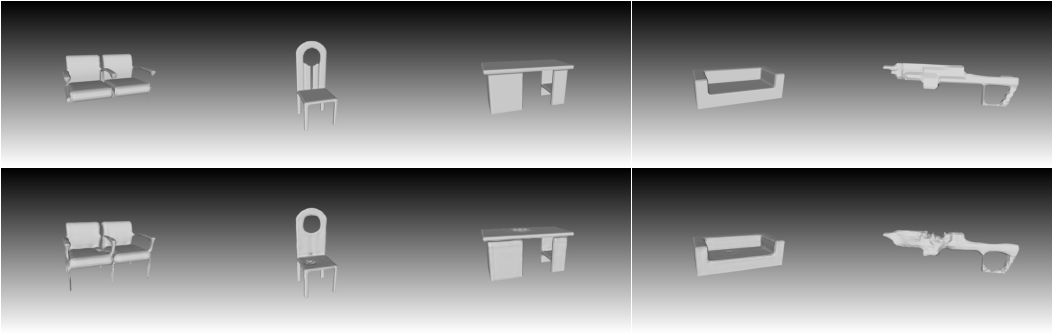
\includegraphics[width=1.0\textwidth]{imgs/vqvae.pdf}
    \caption{The reconstruction results of VQ-VAE on the test set of ShapeNet. The first row is the original object, the second row is the reconstructed object.}
\end{figure}

\begin{figure}[htbp]
    \centering
    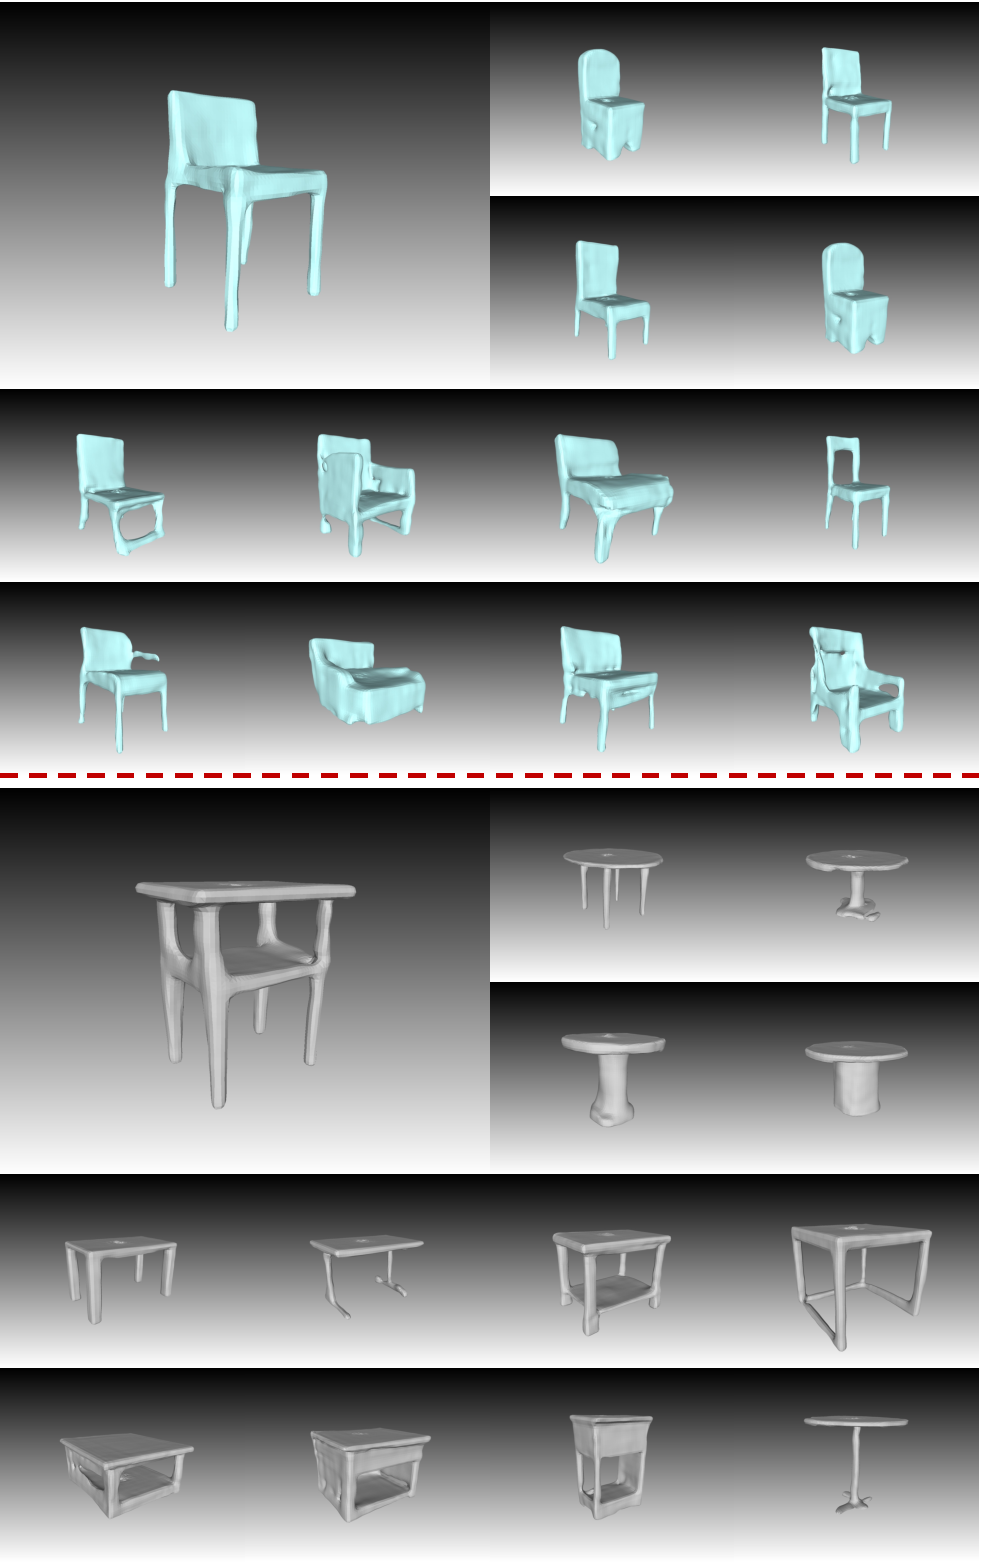
\includegraphics[width=0.85\textwidth]{imgs/table_chair.pdf}
    \caption{Unconditional 3D generation results of table and chair. }
    \label{fig:chairs_table_unconditional} 
\end{figure}
\begin{figure}[htbp]
    \centering
    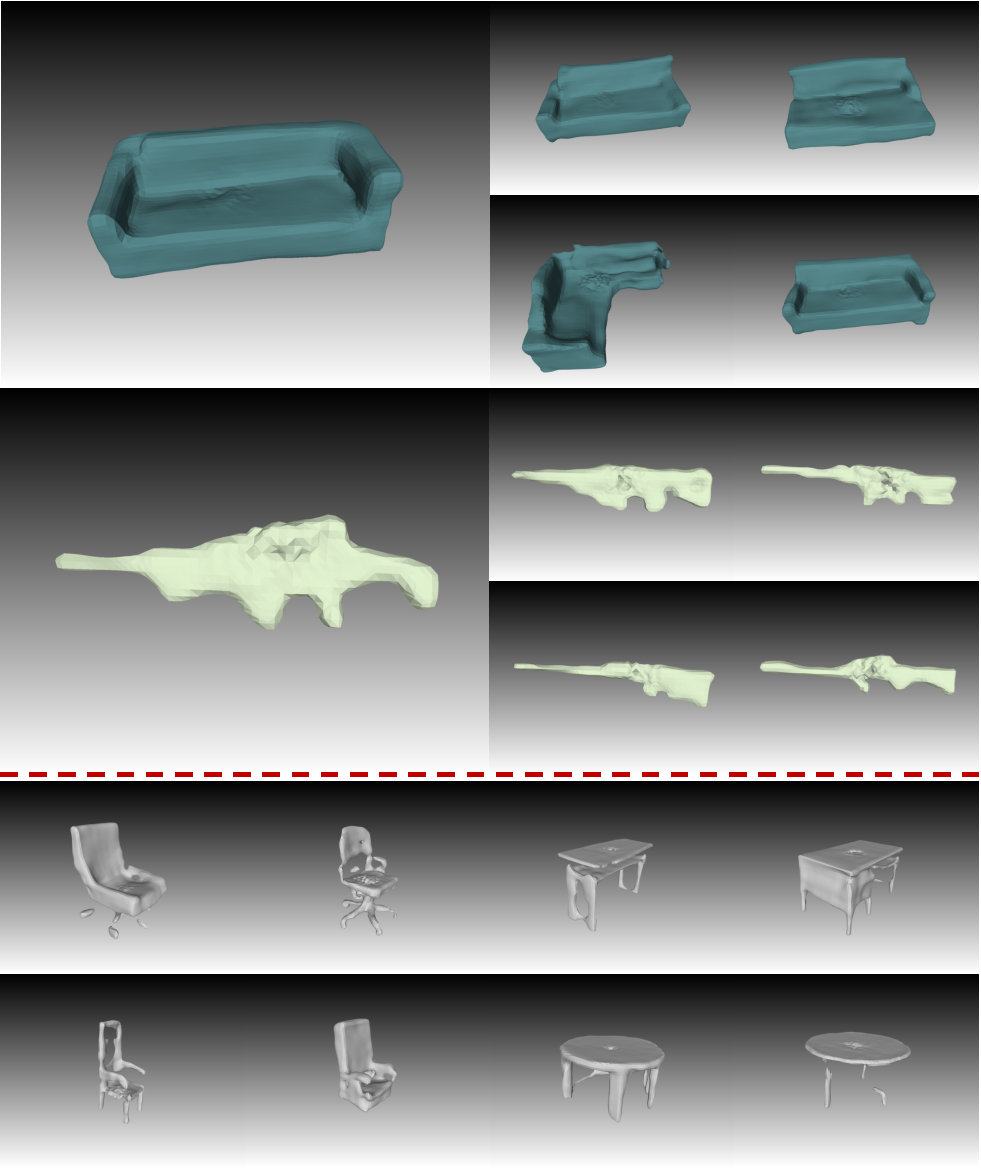
\includegraphics[width=0.9\textwidth]{imgs/other_and_fail.pdf}
    \caption{Unconditional 3D generation results of sofa and rifle. The last two rows are failed cases of table and chair generation, there are some details missing especially in the legs of the table and chair. }
    \label{fig:sofa_rifle_unconditional} 
\end{figure}


\begin{figure}[htbp]
    \centering
    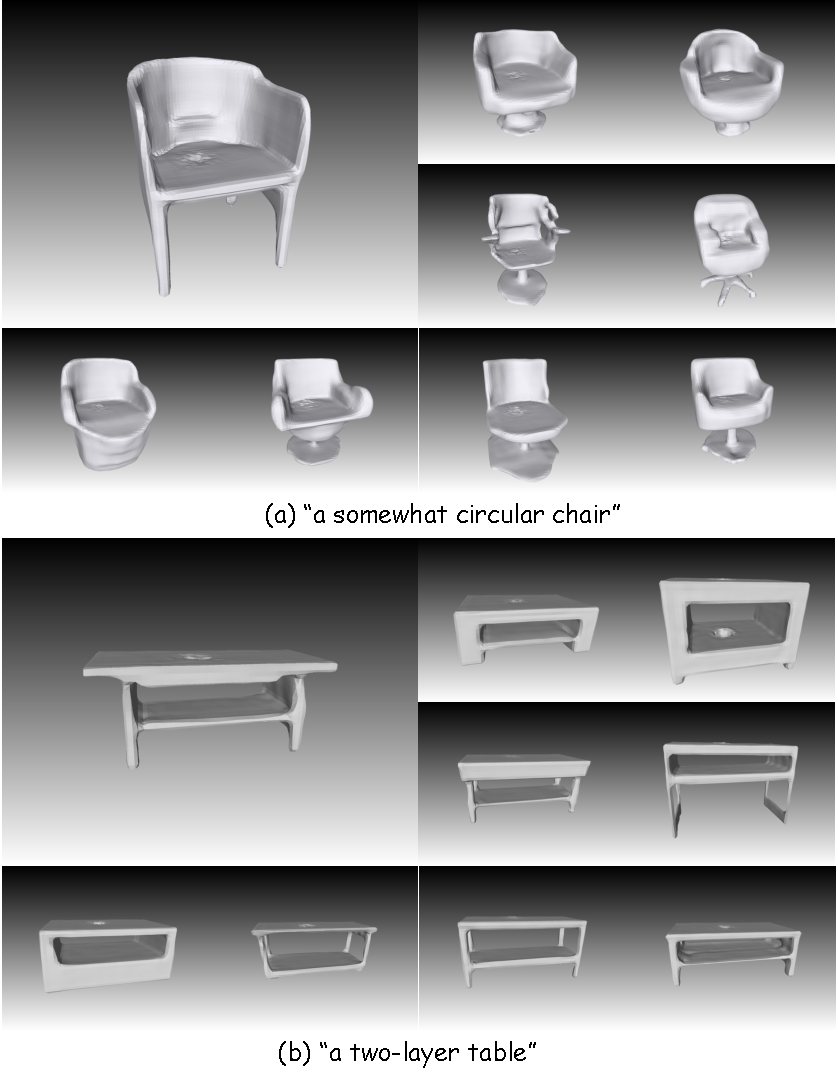
\includegraphics[width=0.8\textwidth]{imgs/result_text_1.pdf}
    \caption{Conditional 3D generation results of table and chair with text prompts.}
    \label{fig:conditional_text_1}
\end{figure}
\begin{figure}[htbp]
    \centering
    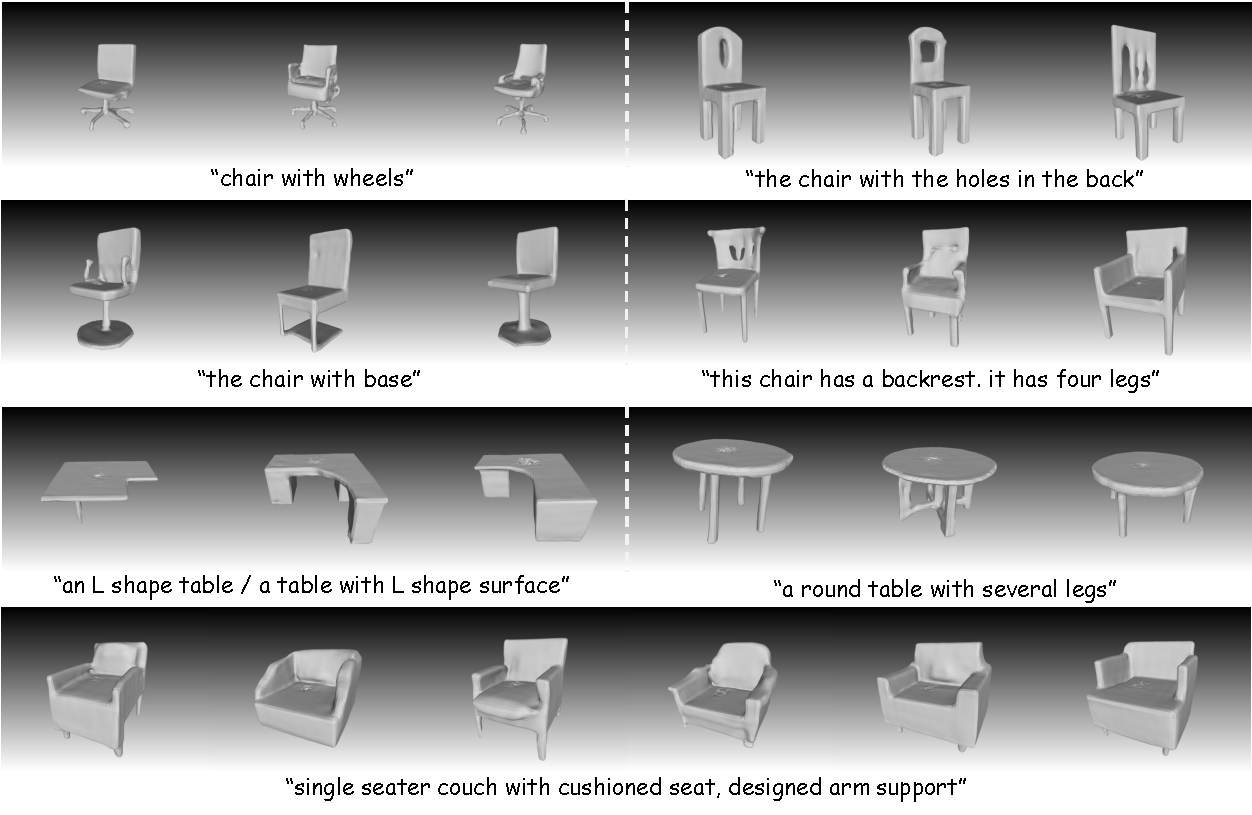
\includegraphics[width=1.0\textwidth]{imgs/result_text_2.pdf}
    \caption{More conditional 3D generation results of table and chair with text prompts.}
    \label{fig:conditional_text_2}
\end{figure}

\section{Conclusion}


\bibliographystyle{plain} 
\bibliography{ref} 

\end{document}